\documentclass[twocolumn]{autart}

%% DOI and ARXIV Commands for Bib Files
% Written by Daniel Herber
% -----------------------------------------------
% one option is to use the 'note' field with this command
% -----------------------------------------------
% for example, if your doi is 10.2514/1.J052182
% then for the citation for the reference in your bib file, use
% note = "\doi{10.2514/1.J052182}",
% -----------------------------------------------
% for example, if your arxiv number is 0706.1234
% then for the citation for the reference in your bib file, use
% note = "\arxiv{0706.1234}",

% requires hyperref package for \href command
\usepackage{hyperref}

% doi command (use in bib file)
\newcommand{\doi}[1]{{doi:~\href{http://doi.org/#1}{#1}}\rmFullStop}

% arXiv command (use in bib file)
\newcommand{\arxiv}[1]{{arXiv:\href{https://arxiv.org/abs/#1}{#1}}\rmFullStop}

% command to remove full stop if the next character
\newcommand*{\rmFullStop}{\rmifnextchar{.}{}{}}

% command to check the next character and replace if present
% \rmifnextchar{X}{[removed text]}{[no X text]}
% if X is the next character, then it is removed and [removed text] is inserted
% otherwise, the character is not removed and [no X text] is inserted
% based on http://tex.stackexchange.com/questions/72827
\makeatletter
\newcommand{\rmifnextchar}[3]{%
  \begingroup
  \ltx@LocToksA{\endgroup#2}%
  \ltx@LocToksB{\endgroup#3}%
  \ltx@ifnextchar{#1}{%
    \def\next{\the\ltx@LocToksA}%
    \afterassignment\next
    \let\scratch= %
  }{%
    \the\ltx@LocToksB
  }%
}
\makeatother
%\RequirePackage{doi}
\usepackage[
	pdftitle={topi.link: The Northern/Southern Ontology},
	pdfsubject={topi.link: The Northern/Southern Ontology},
	pdfauthor={Florian Thiery},
	pdfkeywords={Linked Data, Semantic Reasoning, Vagueness, Conceptual Modeling}
]{hyperref}

\usepackage{graphicx}          % Include this line if your 
                               % document contains figures,
%\usepackage[dvips]{epsfig}    % or this line, depending on which
                               % you prefer.
\usepackage{verbatimbox}

\begin{document}

\begin{frontmatter}
%\runtitle{Insert a suggested running title}  % Running title for regular 
                                              % papers but only if the title  
                                              % is over 5 words. Running title 
                                              % is not shown in output.

\title{topi.link: \protect\\ The Northern/Southern Ontology}
                                               

\author[FT]{Florian Thiery}

\address[FT]{rse@fthiery.de - ORCID: 0000-0002-3246-3531 \protect\\ Research Software Engineer, Mainz, Germany}                                                               

          
\begin{keyword}                             
Linked Data; Semantic Reasoning; Vagueness; Conceptual Modeling. 
\end{keyword}

\begin{abstract}                         

The Linked Geodesy Research Project \textit{topi.link} combines geodesy and Linked Data research questions. Using the Academic Meta Tool (AMT), we have a \textbf{little minion}, which addresses the task of inferencing vague graph data. \textit{topi.link} will give access to the AMT world using toponyms as a graph-based vague topology for these toponyms. This paper demonstrates a very simple example how to model a north/south ontology using AMT.

\end{abstract}

\end{frontmatter}

\section{Introduction}

This example ontology aims the question how to model \textit{relative toponym relations} using the \emph{Academic Meta Tool}\cite{unold_academic_2019} and Linked Data technologies as well as the degree of connection (vagueness). What kind of inferences will result, if we do some reasoning using the AMT JavaScript\cite{thiery_zenodo_3} reasoner? This ontology will help to answer this question. Let us start with a simple imagination: Imagine, we have two Places A and B and we know that A is in the north of B with 70\% (Fig.~\ref{rq1}) and \textit{south} is the inverse of \textit{north} - how will Place C related to A, if B has a degree of connection of about 60\% to Place C (Fig.~\ref{rq2})? 

\begin{figure}[!htb]
\begin{center}
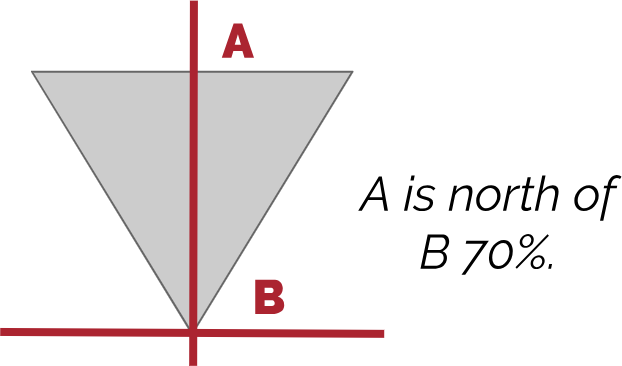
\includegraphics[width=4cm]{question.png}
\caption{Research Question, Florian Thiery [CC BY 4.0]}
\label{rq1}
\end{center}
\end{figure}

\begin{figure}[!htb]
\begin{center}
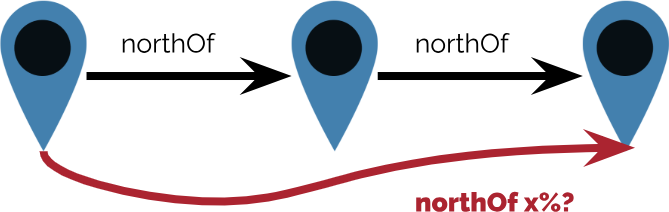
\includegraphics[width=4cm]{question2.png}
\caption{Research Question, Florian Thiery [CC BY 4.0]}
\label{rq2}
\end{center}
\end{figure}

\section{Prefixes}

The following \textit{prefixes} are defined:

\begin{verbnobox}[\tiny\arabic{VerbboxLineNo}\tiny\hspace{1ex}]
@prefix topi: <http://topi.link/ontology/northsouth#> .
@prefix amt: <http://academic-meta-tool.xyz/vocab#> .
@prefix rdfs: <http://www.w3.org/2000/01/rdf-schema#> .
@prefix rdf: <http://www.w3.org/1999/02/22-rdf-syntax-ns#> .
\end{verbnobox}

\section{Academic Meta Tool Scheme}

The used ontology refers to the \textit{Academic Meta Tool Vocabulary} (Penny Edition)\cite{thiery_academic_2018}. An excerpt:

\begin{verbnobox}[\tiny\arabic{VerbboxLineNo}\tiny\hspace{1ex}]
amt:Concept rdfs:subClassOf rdfs:Class .
amt:Role rdfs:subClassOf rdf:Property .
amt:Axiom rdfs:subclassOf rdfs:Class .
amt:InferenceAxiom rdfs:subClassOf amt:Axiom .
amt:IntegrityAxiom rdfs:subClassOf amt:Axiom .
amt:RoleChainAxiom rdfs:subClassOf amt:InferenceAxiom .
amt:InverseAxiom rdfs:subClassOf amt:InferenceAxiom .
amt:DisjointAxiom rdfs:subClassOf amt:IntegrityAxiom .
amt:SelfDisjointAxiom rdfs:subClassOf amt:IntegrityAxiom .
amt:Logic rdfs:subClassOf rdfs:Class .
amt:LukasiewiczLogic rdf:type amt:Logic .
amt:ProductLogic rdf:type amt:Logic .
amt:GoedelLogic rdf:type amt:Logic . 
\end{verbnobox}

\section{The Northern and Southern Places Ontology}

The \textit{Northern and Southern Places Ontology}\cite{thiery_zenodo_1} is defined to show how AMT may help to answer the question shown in section 1. The following sections will explain how it works!

\section{Concepts and Roles}

In our example, we specified one AMT \textit{concept} (Fig.~\ref{concepts}), the general concept of a geographic feature, here the \textit{Place}:

\begin{verbnobox}[\tiny\arabic{VerbboxLineNo}\tiny\hspace{1ex}]
topi:Place rdf:type amt:Concept .
topi:Place rdfs:label "Place" .
topi:Place amt:placeholder "placename" .
\end{verbnobox}

\begin{figure}[!htb]
\begin{center}

\includegraphics[height=3cm]{concepts.png}
\caption{Concepts, Florian Thiery [CC BY 4.0]}
\label{concepts}
\end{center}
\end{figure}

For demonstrating purposes we introduce also two AMT \textit{roles} (Fig.~\ref{concepts}), \textit{northOf} and \textit{southOf} for connecting place nodes with an edge:

\begin{verbnobox}[\tiny\arabic{VerbboxLineNo}\tiny\hspace{1ex}]
topi:northOf rdf:type amt:Role .
topi:northOf rdfs:label "is in the north of" .
topi:northOf rdfs:domain topi:Place .
topi:northOf rdfs:range topi:Place .
topi:southOf rdf:type amt:Role .
topi:southOf rdfs:label "is in the south of" .
topi:southOf rdfs:domain topi:Place .
topi:southOf rdfs:range topi:Place .
\end{verbnobox}

\begin{figure}[!htb]
\begin{center}
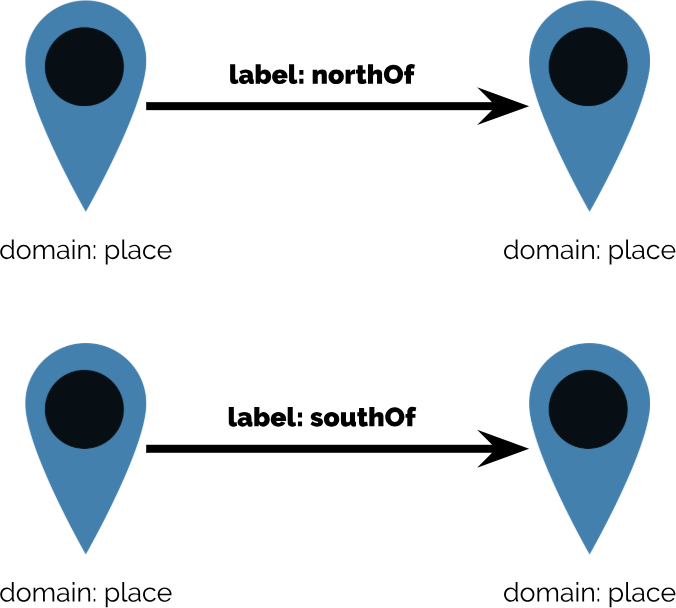
\includegraphics[width=4cm]{roles.png}
\caption{Roles, Florian Thiery [CC BY 4.0]}
\label{roles}
\end{center}
\end{figure}

\section{Axioms}

We also introduce \textit{axioms} to enable reasoning via the AMT JavaScript framework. In this example, we use two types of axioms, the \textit{Role-Chain-Axiom} (Fig.~\ref{rca}) and the \textit{Inverse-Axiom} (Fig.~\ref{ia}). Starting with the simple one, as we all know, \textit{north} is the \textit{inverse} of \textit{south}. In a formal AMT way, the \textbf{antecedent} is \textit{northOf}/\textit{southOf} and the \textbf{inverse} is the opposite role:
 
\begin{verbnobox}[\tiny\arabic{VerbboxLineNo}\tiny\hspace{1ex}]
topi:Axiom03 rdf:type amt:InverseAxiom .
topi:Axiom03 amt:antecedent topi:northOf .
topi:Axiom03 amt:inverse topi:southOf .
topi:Axiom04 rdf:type amt:InverseAxiom .
topi:Axiom04 amt:antecedent topi:southOf .
topi:Axiom04 amt:inverse topi:northOf .
\end{verbnobox}

\begin{figure}[!htb]
\begin{center}
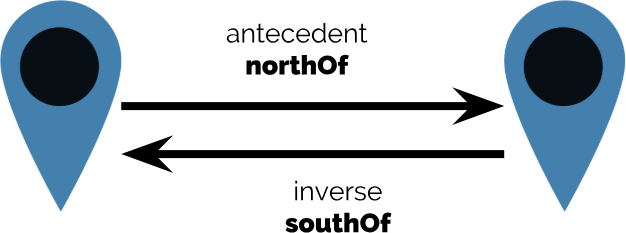
\includegraphics[width=4cm]{axiom_inverse.png}
\caption{Inverse-Axiom, Florian Thiery [CC BY 4.0]}
\label{ia}
\end{center}
\end{figure}

To create role chain \textit{inferences} we use the \textit{AMT Role-Chain-Axiom} where \textbf{antecedent1} is \textit{northOf} or \textit{southOf} and the \textbf{antecedent2} will be the same. In our simple example the \textbf{consequent} will be also the same, here using the \textbf{logic} \textit{ProductLogic}.

\begin{verbnobox}[\tiny\arabic{VerbboxLineNo}\tiny\hspace{1ex}]
topi:Axiom01 rdf:type amt:RoleChainAxiom .
topi:Axiom01 amt:antecedent1 topi:northOf .
topi:Axiom01 amt:antecedent2 topi:northOf .
topi:Axiom01 amt:consequent topi:northOf .
topi:Axiom01 amt:logic amt:ProductLogic .
topi:Axiom02 rdf:type amt:RoleChainAxiom .
topi:Axiom02 amt:antecedent1 topi:southOf .
topi:Axiom02 amt:antecedent2 topi:southOf .
topi:Axiom02 amt:consequent topi:southOf .
topi:Axiom02 amt:logic amt:ProductLogic .
\end{verbnobox}

\begin{figure}[!htb]
\begin{center}
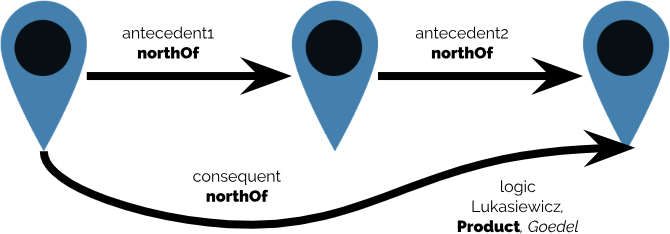
\includegraphics[width=5cm]{axiom_rolechain.png}
\caption{Role-Chain-Axiom, Florian Thiery [CC BY 4.0]}
\label{rca}
\end{center}
\end{figure}

\begin{ack}                               
I would like to thank the Mainz Centre for Digitality in the Humanities and Cultural Studies (mainzed) and R\"omisch-Germanisches Zentralmuseum. In particular Prof. Martin Unold M.Sc (ORCID: 0000-0003-2913-2421), Dr. Kai-Christian-Bruhn (ORCID: 0000-0001-8322-1260) and Dr. Allard Mees FSA (ORCID: 0000-0002-7634-5342).
\end{ack}

\bibliographystyle{IEEEtran}
\bibliography{autosam}

\end{document}